To the best of our knowledge, parametric frailty models are currently especially handled in \proglang{STATA} 
  by means of the \code{streg} command.
With \pkg{parfm}, they are now readily fitted in \proglang{R}.
Further, \pkg{parfm} provides the positive stable frailty distribution 
  which is presently unavailable in \proglang{STATA}.
Actually, except for a \proglang{SAS} macro, \code{ps_frail}, 
  developed by \cite{ShuKlein99} in the semi-parametric setting, 
  we are not aware of another package that provides the positive stable frailty distribution.

% % % Parfm package features % % % 
The \pkg{parfm}~package is flexible and easy to use. 
It provides five distributions for the baseline hazard and three frailty distributions.
Parameter estimation is done by maximising the marginal log-likelihood given in Equation~\ref{eq:loglik.marg}.
The \code{optim()} function is employed, 
  and its \code{method} option is passed to \code{parfm()} (with \code{method="BFGS"} by default).
If not specified in the \code{inip} option, 
  initial values for all but the heterogeneity parameter are obtained by fitting 
  an unadjusted (i.e., without frailty) parametric proportional hazards model 
  using the \code{phreg()}~function from the \pkg{eha}~package \citep{R:eha}.
The initial heterogeneity parameter can also be specified by the user via the \code{iniFpar} option;
  otherwise it is set to $1$ when frailties follow a gamma or an inverse Gaussian distribution, 
  or to $1 \slash 2$ when they follow the positive stable distribution.

% % % No frailty estimation % % % 
Additionally, when \code{frailty="none"}, \code{parfm()} fits the unadjusted parametric proportional hazards model,
  similar to \code{survreg()} (from the \pkg{survival} package) or to \code{phreg()}.
However, \code{survreg()} returns the parameter estimates in the log-linear model 
  and \code{phreg()} uses yet another parametrisation (see the documentation).
Often, the user has then to transform back the parameters 
  and to employ the delta method in order to get estimates for the standard errors.
The \code{parfm()} function directly uses the proportional hazards representation.

% % % Problems % % % 
Nonetheless, \pkg{parfm} might reach its limits when at least one $d_i$,
  the number of events in the $i$-th cluster, $i \in \{ 1, \ldots{}, G \}$, is very large.
% 
% % PS
First, consider the positive stable distribution and observe that, 
  for a fixed value of $m \in \{1, \ldots, q-1\}$, $\Omega_{q, m}$ rapidly grows as $q$ increases; 
  see Equations~\ref{eq:PSOmegas}.
At the extreme, some of them might exceed the largest representable number in \proglang{R}.
These are then stored as \code{Inf}. 
This, in turn, prevents the marginal log-likelihood~\ref{eq:loglik.marg} to be evaluated and hence maximised.
On a side note, also the \proglang{SAS} macro \code{ps_frail} that implements the EM algorithm to fit the semi-parametric positive stable frailty model 
	has analogous difficulties when the number of events is large (or even moderate).
The following ad-hoc solution is implemented in \pkg{parfm}:
  in order to keep the polynomials $\Omega_{q, m}$'s reasonably small, 
  they are divided by some factor $10^{K}$ which does not change the marginal log-likelihood
	except for an additive constant (equal to $s \times K \times \log ( 10 )$).
The value of $K$ is specified via the \code{correct}~option (default is \code{correct=0}, i.e., no correction)
	and \code{parfm()} returns the re-adjusted log-likelihood value.
That solution serves the purpose for moderately large values of $d_{i}$ 
  (say up to about $200$ events per cluster according to our experience, 
  but it depends on the data, on the other parameters,
  and on the hardware characteristics).
%   
% % IG
With the inverse Gaussian distribution, 
  the Bessel function $K_{q - 1 \slash 2} ( z )$ in Equation~\ref{eqn:ingau} raises the same problem.
Indeed, it explodes when $z$ is small relative to $q$; see Figure~\ref{fig:bessel}.
Currently, that distribution should, therefore, preferably be avoided when there are very 
  large values of $d_{i}$ (say above $200$ events per cluster according to our experience,
  but, again, it depends on the data, on the other parameters and on the hardware characteristics).
Moreover, $K_{q - 1 \slash 2} ( z )$ rapidly goes to zero as $z$ increases. 
So, in case of very small apparent heterogeneity, $\theta \rightarrow 0$ which implies $z \rightarrow \infty$, 
	$K_{q - 1 \slash 2} ( z )$ might be stored as $0$ in \proglang{R} and hence $\log( K_{q - 1 \slash 2} ( z ) )$ 
	cannot be computed.
However, 
  as this problem occurs in the case of very small heterogeneity,
  this would rather suggest to fit the model with \code{frailty="none"}.	
  % 
  \begin{figure}[htbp]
  \centering
  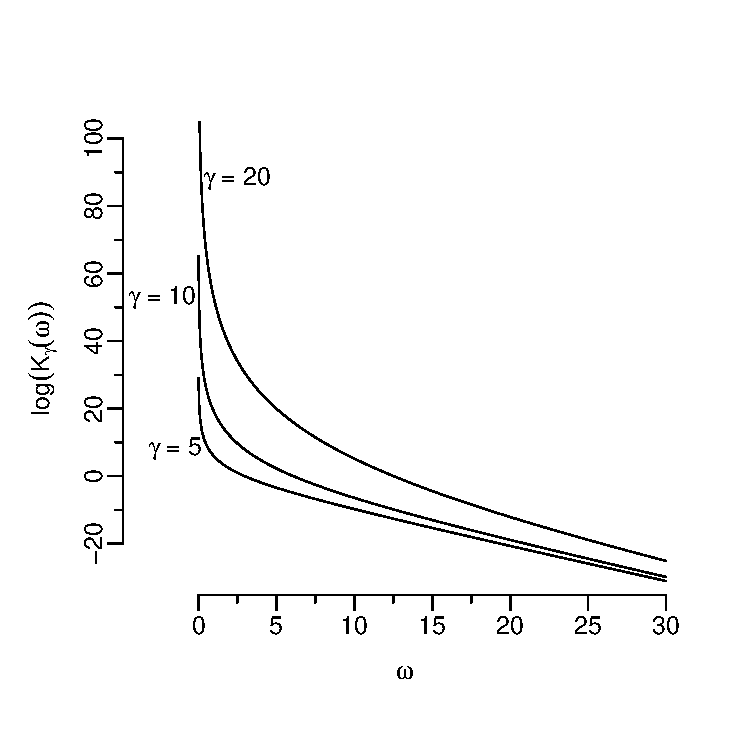
\includegraphics[width=.6\textwidth]{./graphs/bessel.pdf}
  \caption{The logarithm of the Bessel function, $\log ( K_{\gamma} ( \omega ) )$, versus $\omega$ for different values of $\gamma$.} 
  \label{fig:bessel}
  \end{figure}
  % 
% 
% % gamma
When frailties are gamma distributed,
  which is by far the most popular assumption in common practice, 
  the quantities involved in Equation~\ref{eqn:gamma} do not raise any worry.
In practice, even when dealing with datasets with huge numbers of events per cluster,
  there is no real risk of exceeding the range of floating-point numbers.